\documentclass[12pt,a4paper]{article}

% include standard packages:
\usepackage{graphicx, epstopdf} % for e.g. MATLAB-Grafiken im .eps-format
\graphicspath{{./img/}} % default folder for figures
\usepackage[tmargin=1in,bmargin=1in,lmargin=1.25in,rmargin=1.25in]{geometry} % MSWord-Format
\setlength{\parindent}{0em} % keine Einrueckungen, sonst \noindent

\usepackage{xcolor}
\usepackage{hyperref} % [colorlinks,linkcolor=black,citecolor=black,urlcolor=black] % customize references
\usepackage{amsmath, amsfonts, amssymb, amsthm} % enhanced math writing

\usepackage{listings, lstautogobble} % adding code listing support
\newcommand*\listingspath[1]{\lstset{inputpath=#1}}
\listingspath{./codes/} % default folder for codes

\usepackage{float} % improved inteferce of floating objects (e.g. \floatplacement{figure}{H})
\usepackage{sectsty} % applay different fonts for a section
\usepackage{eso-pic} % backround image e.g.

% Umlaute-Encoding und Standardschrift einstellen:
\usepackage[ngerman]{babel}
\usepackage[utf8]{inputenc}
\usepackage[T1]{fontenc}
\usepackage{lmodern}

% uncomment the following 2 lines to use Arial
%\usepackage{helvet}
%\renewcommand{\familydefault}{\sfdefault}

%\renewcommand{\contentsname}{Inhaltsverzeichnis} % Rename listings
%\renewcommand{\lstlistlistingname}{Codelisting}
%\renewcommand{\listfigurename}{Abbildungsverzeichnis}
%\renewcommand{\listtablename}{Tabellenverzeichnis}

% Title page configuration
\title{Project Description: \\ Temperature-Measuring and Visualization System}
\author{Jonas Berger}
\date{Datum: 10.11.2021}

\begin{document}
\maketitle

%\renewcommand{\abstractname}{Abstract} % if german-babel used change Abstractname here
%\begin{abstract} % make Abstract
	%\noindent
	\section{Einleitung}
	Dieses Dokument soll das Projekt "Temperature-Measuring and Visualization System"\space beschreiben. Dabei zeigt das nachfolgende Blockschaltbild \ref{figure:1} alle verwendeten Bauteile, Sensoren und Anzeigen mit den entsprechenden Bussystemen bzw. Ansteuerungen:
	\begin{figure}[H]
		\centering
		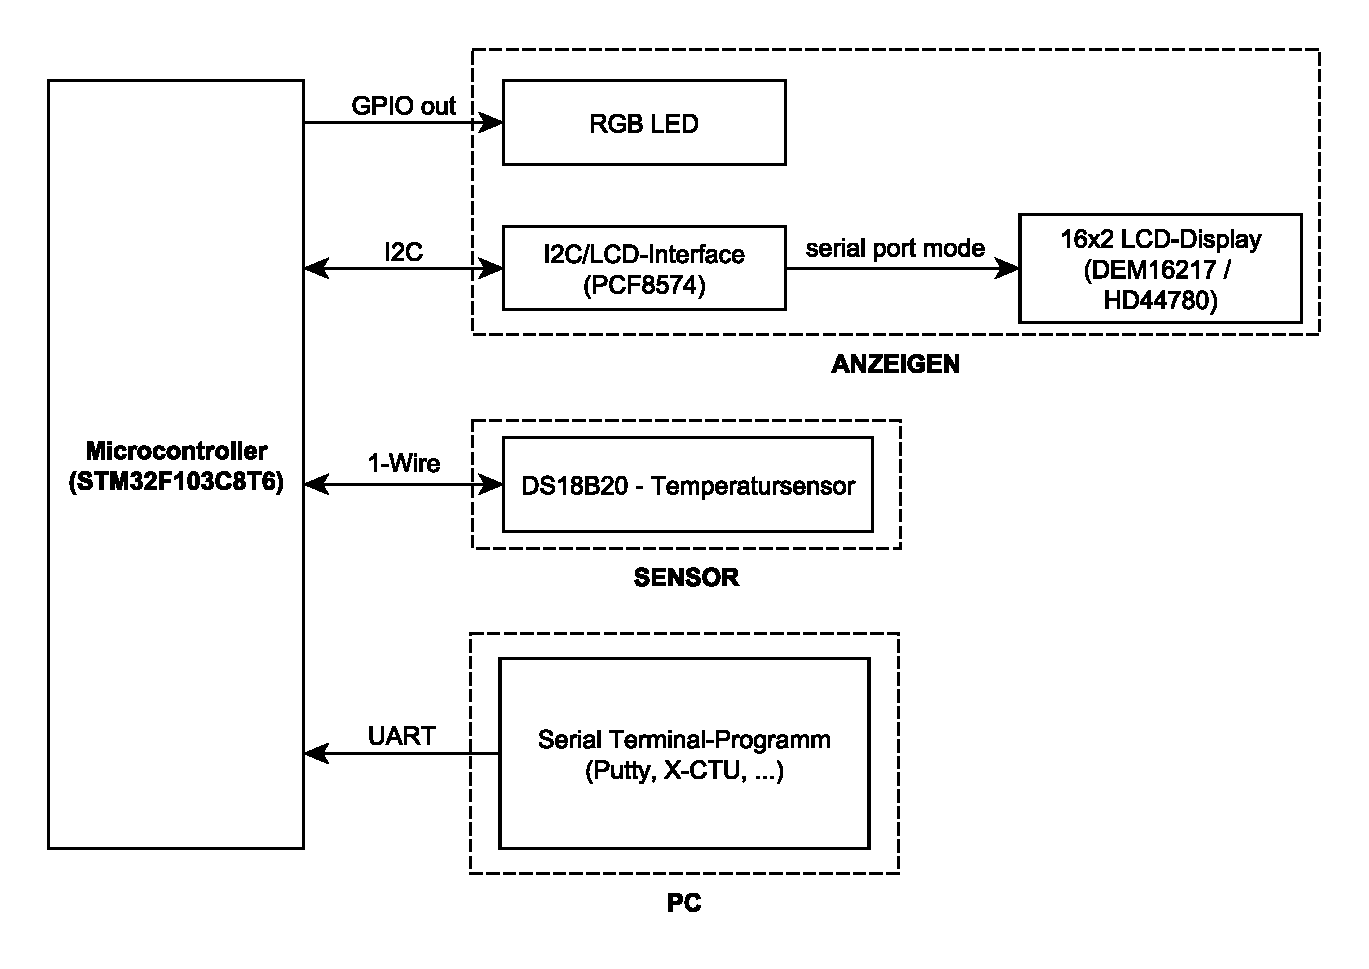
\includegraphics[width=0.9\linewidth]{Project_Mockup_V05}
		\caption{Blockschaltbild}
		\label{figure:1}
	\end{figure}
	\pagebreak
	
	\section{Aufgabenstellung}
	Zunächst soll die aktuelle Temperatur mit dem DS18B20-Temperatursensor über das 1-Wire-Protokoll ausgelesen werden. Dieser Wert soll auf ein 16x2 LCD-Display ausgegeben werden. \\
	Jedoch wird der Wert nicht direkt vom Microcontroller an das Display übertragen, sondern wird an den $\mathrm{I^{2}C}$-to-LCD Interface-Baustein (PCF8574) via $\mathrm{I^{2}C}$ gesendet. Damit wird ein hoher Verbrauch von Portleitungen des Microcontrollers zur Ansteuerung des Displays vermieden. \\
	\\ Ein weiteres Feature ist die Einstellung einer Solltemperatur via UART über einen angeschlossenen PC mit einem Serial-Terminal-Programm. Dieser Wert wird ebenfalls am LCD-Display angezeigt. \\
	Sollte sich die gemessene Temperatur innerhalb einer gewissen Toleranz befinden leuchtet eine RGB-LED grün. Ansonsten werden Abweichungen vom Sollwert stufenweise rot-grün bis rot angezeigt.
	
	\section{Verwendete Hardware}
	Folgende Hardware wird für das Projekt benötigt:
	\begin{itemize}
		\item STM32F103C8T6-Microcontroller
		\item 16x2 LCD-Display (z.B. HD44780, DEM16217, ...)
		\item I2C/LCD-Interface Baustein (verwendet PCF8574-Chip)
		\item RGB-LED (KY-016)
		\item DS18B20 1-Wire-Temperatursensor
		\item PC mit Serial-Terminal-Programm (z.B. Putty, X-CTU, ...)
	\end{itemize}

\end{document}